Our application is modelled using a \gls{moc} or a programming model that allows timing analysis.  
Our model should capture dynamic behaviour and scenario-awareness. 
This enables us to model and analyse execution time variations that happen at runtime due to either image workload variations and/or platform load. 
We assume that \gls{wcet} estimates of task workloads are given for a platform or can be computed.

A \gls{moc} is required to compute the parameters relevant for the control design - the sampling period $h$ and the sensor-to-actuator delay $\tau$.
However, the challenge now is: How to accurately determine $h$ and $\tau$ at design time for a multiprocessor, possibly heterogeneous, platform implementation?
The choice of binding and scheduling of tasks on the platform determines $h$ and $\tau$.

\subsection{\Acrfull{sadf}}
\label{sec:ch5_sadf}
We choose \gls{sadf}~\cite{theelen2006scenario} as the
formal \gls{moc} for our application as it enables us to: i) model dynamic behaviour, analyse timing, and optimally map application tasks to the platform for maximising the effective utilisation of allocated resources, ii) relate throughput of the dataflow graph to the sampling period, and thus combine dataflow analysis and mapping with control design parameters and \gls{qoc}, and iii) to efficiently implement a runtime mechanism that manages necessary dynamic reconfiguration between system scenarios.

Following the formalisation of~\cite{ara2018scalable}, an \gls{sadf} model is a tuple
($\Scenarios,\ \fsmsadf$), where
\begin{itemize}
  \item $\Scenarios \ =\ \{\scenario_i\ \mid\ \scenario_i =\ (\aWorkload_i,\SDFG_{i}),\ \aWorkload_i \in \setW\}$ is a set of scenarios being a set of pairs of workloads $\aWorkload_i$ and their corresponding \glspl{sdfg} $\SDFG_{i}$;
  \item the ($\omega$-)language $\fsmsadf$ describes a set of infinite scenario sequences represented using $\omega$-regular expressions of scenarios $\scenario_i \in \Scenarios$.
\end{itemize}

Here, the workload refers to the image workload, i.e., the number of features in the image that should be processed. For example, more features in an image imply a higher workload.
We assume that workloads are totally ordered, i.e., for any two workloads $\aWorkload_i$ and $\aWorkload_j$, either $\aWorkload_i\leq \aWorkload_j$ or $\aWorkload_j\leq \aWorkload_i$.
Ordering the workloads helps to prune the state-space for system-scenario identification (explained later in Section \ref{sec:ch5_ch5_sys_scenario}).

An \gls{sdfg}~\cite{lee1987synchronous} is a tuple $\SDFG = (\Actors,\ \Channels,\ \actorET,\ \ratesSDFG_p,\ \ratesSDFG_c,\ \initialTokens)$
where $\Actors$ is a finite set of actors, $\Channels \subseteq \Actors^2$ the set of channels,
$\actorET \ :\ \Actors \rightarrow \R_{\geq 0}$ returns for each actor its associated firing delay. The firing delay models the time it takes to execute (fire) an actor. If an actor models a computational task, the firing delay typically models the (worst-case) execution or response time of that task.
$\ratesSDFG_p \ :\ \Channels \rightarrow \N_{> 0}$ is a function that returns for each channel its production rate,
$\ratesSDFG_c \ :\ \Channels \rightarrow \N_{> 0}$ is a function that returns for each channel its consumption rate,
$\initialTokens \ :\ \Channels \rightarrow \N_{0}$ returns for each channel its number of
initial tokens. When actors of an \gls{sdfg} fire, they consume and produce tokens according to the specified consumption and production rates. They can only fire if sufficient tokens are available on their input channels.

A \emph{repetition vector} $\repetitionVector$ of an \gls{sdfg} $\SDFG$ is a function $\repetitionVector: \Actors \longrightarrow \N_0$ such that for every channel $c=(a_m,a_n)\in \Channels$, $\ratesSDFG_p(c) \times \repetitionVector(a_m)=\ratesSDFG_c(c) \times \repetitionVector(a_n)$.
A repetition vector $\repetitionVector$ for an \gls{sdfg} $\SDFG$ is called non-trivial iff for all $a_m \in \Actors$, $\repetitionVector(a_m) > 0$.
An \gls{sdfg} is called consistent iff it has a non-trivial repetition vector. 
For a consistent \gls{sdfg}, the unique smallest non-trivial repetition vector is designated as the repetition vector $\repetitionVector$ of the \gls{sdfg}. 
An \gls{sdfg} \emph{iteration} is a minimal non-empty set of actor firings that has no net effect on the token distribution in the graph. For a consistent \gls{sdfg}, for all $a_m\in \Actors$, the set contains $\repetitionVector(a_m)$ firings of $a_m$. 
For the scope of this work, we assume that the \gls{ibc} application model, which is an \gls{sadf}, can only have consistent \glspl{sdfg} and the \glspl{sdfg} are deadlock-free. These assumptions can be checked efficiently and are valid as any \gls{sdfg} which is inconsistent or deadlocks is not useful in practice. 

\begin{figure}
    \centering
    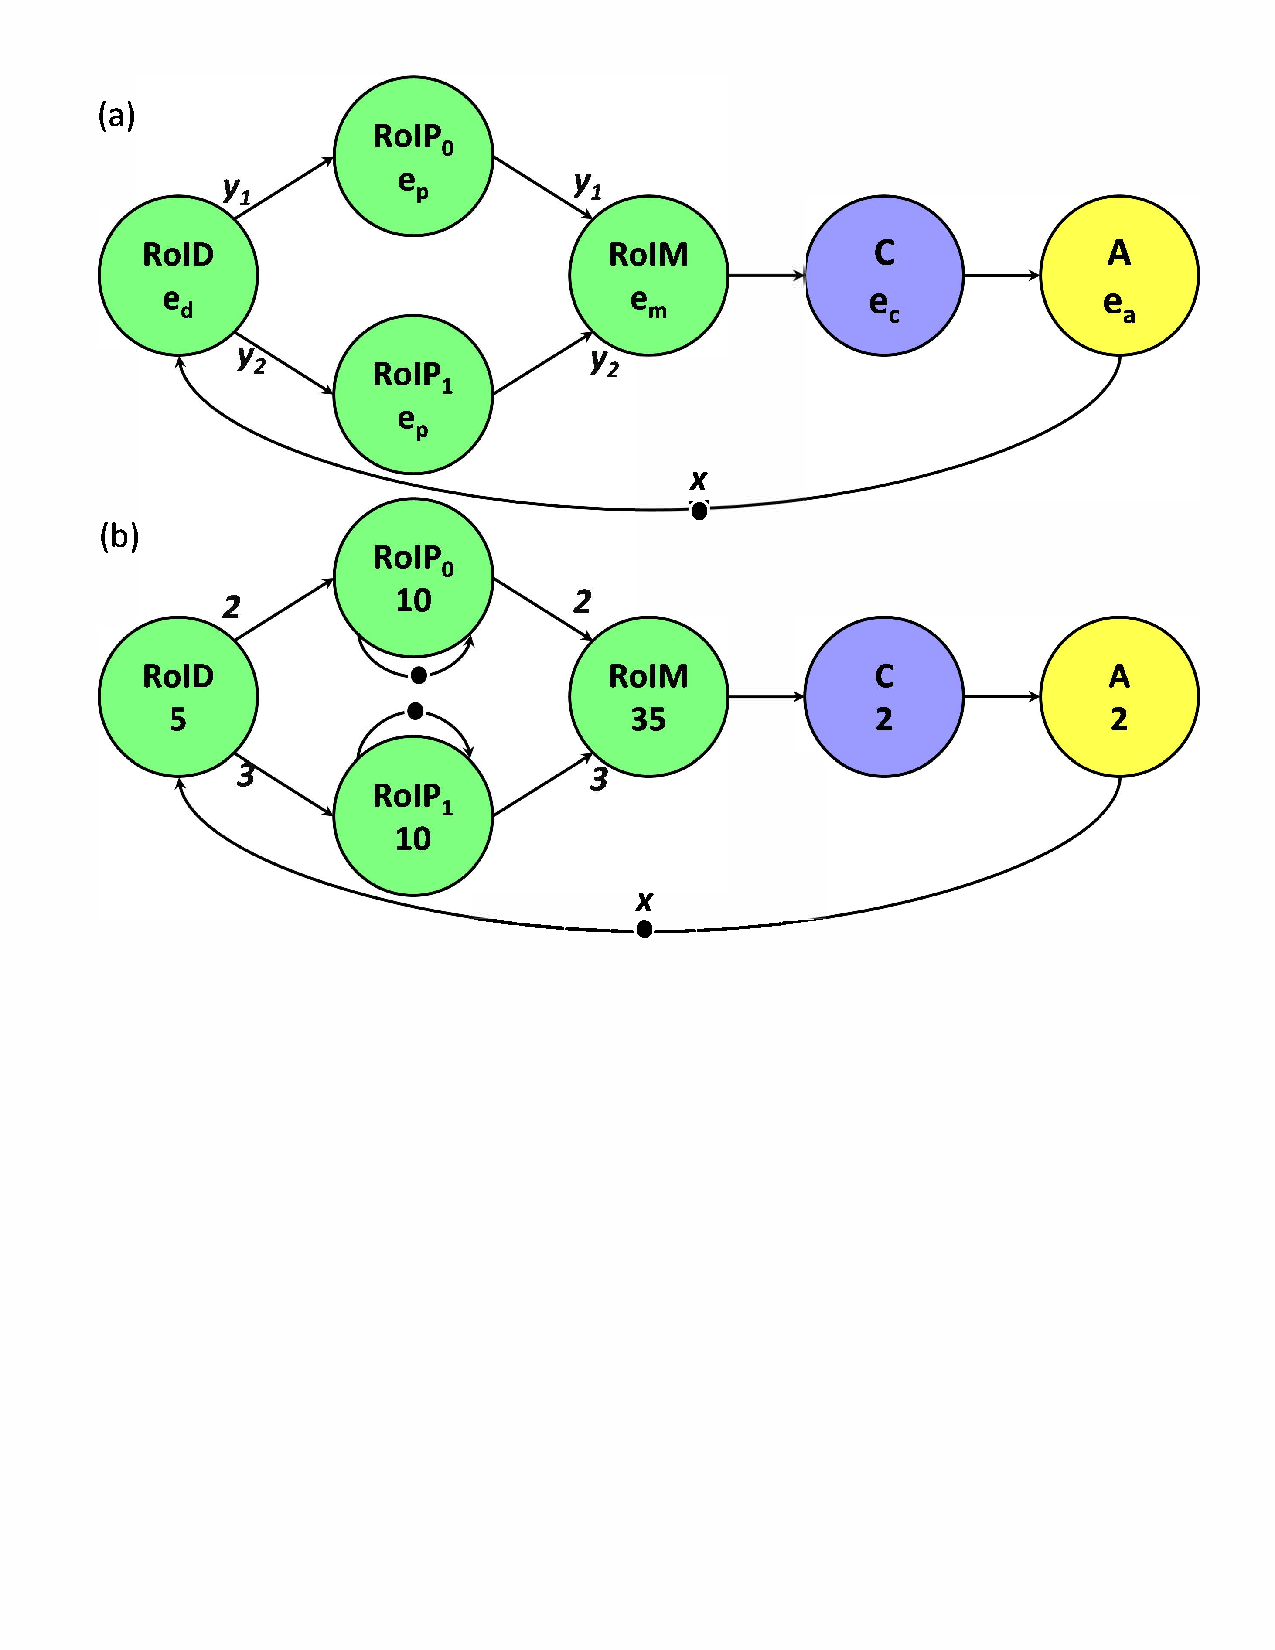
\includegraphics[scale=0.375]{images/sadf.pdf}
    \vspace{-14em}
    \caption{\Gls{lkas} dataflow model, assuming two allocated processors and hence two RoIP actors: (a) application model; (b) (simplified) binding-aware SDFG.}
    \label{fig:ch5_SADF}
\end{figure}

The \gls{sadf} model for our \gls{lkas} \gls{ibc} application is illustrated in Fig.~\ref{fig:ch5_SADF}(a).
The sensing and processing algorithm receives the camera image frames and detects the regions-of-interest (RoID) in the frames. 
In this case, the workload is related to the number of \glspl{roi}.
The detected \glspl{roi} can be processed in parallel on a multiprocessor platform. The number of allocated processors for our application determines the number of \gls{roi} processing (RoIP) actors in our model. In this case, we have two allocated processors and hence two RoIP actors. The total number of \gls{roi} detected by RoID determines the workload $\aWorkload_i$, i.e., $\aWorkload_i=y_{1}+y_2$.
The parameters $y_1$ and $y_2$ determine how many \gls{roi} need to be allocated to the individual processors and are the rates for the corresponding scenario $\scenario_i$.
Note that the workloads here are totally ordered as they are related to the number of \glspl{roi}.
Rates are annotated with the channels, where rates of 1 are not shown explicitly. The workloads translate to variable token production and consumption rates in the scenario \glspl{sdfg}.
Note that the sensor-to-actuator delay and sampling period vary based on the value of $y_1$ and $y_2$. After processing the \gls{roi}, the data is merged and the controller state (the lateral deviation $\yL$ in our \gls{lkas} case study) is computed by the \gls{roi} merging (RoIM) task. The control algorithm (\taskC) then computes the controller input $u[k]$ (steering angle $\delta_f$ in our \gls{lkas} case study) and feeds it to the actuation (\taskA) task. 

Each workload $\aWorkload_i$ in an \gls{sadf} is associated with an \gls{sdfg} $\SDFG_i$. 
An \gls{sdfg} instance of Fig.~\ref{fig:ch5_SADF}(a) is obtained by assigning values to parameters $\actorET_j$ (the actor execution times) and $y_k$. 
E.g., assigning $y_1=2,\ y_2=3,\ \actorET_d=5,\ \actorET_p=10,\ \actorET_m=7\times(y_1+y_2)=35,\ \actorET_c=2,\ \actorET_a=2$ gives the \gls{sdfg} for a workload of 5 \glspl{roi} for mapping to two processors.
The actors of $\SDFG_i$ are $\Actors_i=\{\text{RoID}, \text{RoIP}_0, \text{RoIP}_1, \text{RoIM}, \text{\taskC}, \text{\taskA}\}$. Fig.\ \ref{fig:ch5_SADF}(b) illustrates an SDFG as it is derived from the model structure of Fig.\ \ref{fig:ch5_SADF}(a). (This is actually a binding-aware SDFG, as explained later.) The set of channels of $\SDFG_i$, $\Channels_i$, is shown as dependencies in the figure. Compared to the model of Fig.\ \ref{fig:ch5_SADF}(a), the SDFG of Fig.\ \ref{fig:ch5_SADF}(b) has two additional channels, self-loop channels for the RoIP actors. There are three initial tokens, one on the channel from actor \taskA\ to RoID and two on the self-loop channels for the RoIP actors. The self-loop channels and their initial tokens capture the fact that each of the RoIP actors is executed sequentially on its allocated processor.
The workload scenarios are defined based on $\aWorkload_i$ and the parameters that change for the corresponding $\SDFG_i$ are $y_1,\ y_2,$ and $\actorET_m=7\times (y_1+y_2)$. All other aspects of the $\SDFG_i$ are the same for all scenarios.
There is one (labelled) initial token $x$ in the channel from actor \taskA\ to RoID.
For the \gls{sadf} model in Fig.~\ref{fig:ch5_SADF}, for each scenario $\aWorkload_i$,
the corresponding \gls{sdfg} $\SDFG_i$ has repetition vector $\repetitionVector_i= \left[ \begin{array}{cccccc} 1 & y_1 & y_2 & 1 & 1 & 1  \end{array} \right]$, where $y_1$ and $y_2$ represent the firing rates of the two actors RoIP shown in Fig.~\ref{fig:ch5_SADF}. A word from the \gls{sadf} language $\fsmsadf$ now specifies a sequence of iterations of the corresponding scenario \glspl{sdfg}.

The state-of-the-art \gls{sadf} analysis uses (max, +) algebra~\cite{baccelli1992synchronization}.
The definitions needed for our analysis are summarised in the following paragraphs. For detailed explanations and analysis methods, the reader is referred to~\cite{ara2018scalable}.

A time-stamp vector $\maxplusLambda{0}{}$ captures the availability times of a subset of initial tokens, called the \emph{labelled} initial tokens.
The production times $ \maxplusLambda{1}{}$ of the labelled \emph{final} tokens resulting from the execution of a scenario $\scenario$ are then captured by Eq.(~\ref{eq:ch5_max-pluslambda}).
\begin{equation}
\label{eq:ch5_max-pluslambda}
  \maxplusLambda{1}{} = \maxplusMatrix_{\scenario} \maxplusLambda{0}{},
\end{equation}
where $\maxplusMatrix_{\scenario}$ is the scenario (or state) matrix of $\scenario$.
We assume that the labelled initial and final tokens are the same, and that the execution of a scenario corresponds to one iteration of the corresponding \gls{sdfg}. For the scenario \gls{sdfg} corresponding to 5 RoI, introduced above in Fig.\ \ref{fig:ch5_SADF}(b), the initial token on channel \taskA-RoID labeled $x$ is a labelled token and  $\maxplusLambda{0}{}=\left[ 0\right]$. 
$\maxplusMatrix_{\scenario}=\left[ \actorET_d+ \max (y_1,y_2)\times \actorET_p+\actorET_m+\actorET_c+\actorET_a\right]$ $=\left[ 74\right]$ and $\maxplusLambda{1}{}=\left[ 74\right]\left[ 0\right]=\left[ 74 + 0\right]=\left[ 74\right]$. 

$\maxplusMatrix_{\scenario}$ is used to determine the evolution of any scenario sequence. Labelled final tokens of one scenario are the initial tokens of the next scenario execution. E.g., if $\scenario^\omega$ is the infinite repetition of scenario $\scenario$, then the production times of the labelled tokens after the execution of the $k^{th}$ scenario in the sequence are given by:
%
\begin{equation}
\label{eq:ch5_max-plus-kth}
  \maxplusLambda{k}{}= \maxplusMatrix_{\scenario} \maxplusLambda{k-1}{} = \maxplusMatrix_{\scenario}^k \maxplusLambda{0}{} 
\end{equation}

For all scenarios $\scenario \in \Scenarios$, we can construct $\maxplusMatrix_{\scenario} \in \R_{-\infty}^{\initialTokens(\scenario) \times \initialTokens(\scenario)}$ following the procedure of~\cite{siyoum2014symbolic}.
Here, $\initialTokens(\scenario)$ is the total number of labelled initial tokens (in all channels) for scenario $\scenario$ and $\R_{-\infty}=\R\cup\{-\infty\}$ is the domain of (max, +) algebra.

Further, we need to analyse the production times of \emph{outputs}, i.e., the relevant information produced, during the execution of a scenario sequence.
Let the function $\FnScenarioToOutput:\Scenarios \rightarrow \N\ \cup\ \{0\}$ map each scenario to the number of outputs produced in that scenario.
The output production times of the scenario sequence $\scenario^\omega$ can be computed as,
\begin{equation}
 \label{eq:ch5_prod-times}
  \prodTime_k = \maxplusMatrixOutput_{\scenario} \maxplusLambda{k}{}=\maxplusMatrixOutput_{\scenario}\maxplusMatrix_{\scenario}^k \maxplusLambda{0}{} 
\end{equation}

where $\prodTime_k$ are the times at which the outputs in the $(k+1)^{th}$ iteration are produced and where $\maxplusMatrixOutput_{\scenario} \in \R_{-\infty}^{\FnScenarioToOutput(\scenario) \times \initialTokens(\scenario)}$ is the output matrix of the scenario $\scenario$ that captures the relation between the state vector and the production times of the $\FnScenarioToOutput(\scenario)$ outputs. 
Note that the first output production times are given by $\prodTime_0$. 
The $\maxplusMatrixOutput_{\scenario}$ matrices can be computed in a similar way as the state matrices.

For the \gls{lkas} scenarios, the output is produced by the actor \taskA, meaning that the output production time is equal to the production time of the token on the channel from \taskA\ to RoID. This means that $\maxplusMatrixOutput_{\scenario}=\left[ 74\right]$ and the production time of the first output $\prodTime_0=\left[ 74\right]\left[ 0\right]=\left[ 74\right]$.

We quantify the throughput $\FnThroughput$ of a given scenario sequence from the language $\fsmsadf$ of an \gls{sadf} model by the average number of outputs produced per time unit during the execution of that sequence.
The throughput of an \gls{sadf} for an infinite scenario sequence $\bar{\scenario}$ is defined as follows.
\begin{equation}
\label{eq:ch5_maxplus-throughput}
  \FnThroughput (\bar{\scenario}) = \lim\limits_{n \to \infty} \text{sup } \frac{\sum_{i=1}^{n} \FnScenarioToOutput (\bar\scenario_i)}{\norm{\maxplusLambda{n}{}}}
  %\nonumber
\end{equation}
where $\bar\scenario_i$ refers to the $i^{th}$ symbol in sequence $\bar\scenario$ (a scenario), and $\norm{\maxplusLambda{n}{}}$ is equal to the maximum entry in the vector $\maxplusLambda{n}{}$.
For the infinite execution of the 5 \gls{roi} scenario \gls{sdfg}, the throughput is $\frac{1}{74}$.
We omit the details of the computation, referring the reader to~\cite{ara2018scalable}.
 
\vspace{1ex}
For the \gls{sadf} models in our basic \gls{spade} flow, we assume the following.
\vspace{-1ex}
\begin{itemize}
  \item Throughput is inversely monotonic for our \gls{sadf} model for different workloads. This assumption can be relaxed if we do a brute-force exploration for system-scenario identification (explained later in Section \ref{sec:ch5_ch5_sys_scenario}). This assumption is required as we do not have a \gls{dse} step in the basic \gls{spade} flow. The monotonicity is guaranteed by the following:
  \begin{enumerate}
      \item The set of actors $\Actors$ is the same for all scenarios, i.e. $\Actors_{i}=\Actors_{j}$, where $\Actors_{i}$ and $\Actors_{j}$ are the sets of actors of $\SDFG_i$ and $\SDFG_j$ respectively.
      \item $\aWorkload_i \leq \aWorkload_j \implies \frac{1}{\FnThroughput(\SDFG_i)} \leq \frac{1}{\FnThroughput(\SDFG_j)}$.
  \end{enumerate}
   \item The sensing task is not pipelined, i.e., the control is sequential. This is guaranteed by having a channel with only one initial token from the actuation task to the start of the sensing task in our \gls{sadf} model (as in the example).
\end{itemize}
 Both these assumptions are relaxed in Chapter~\ref{chap:pipelined_parallelism}. 

\subsection{System mapping and mapping configurations}
System mapping refers to the binding of the application (modelled as an \gls{sadf} model) to the given platform (modelled as a platform graph) allocation. 
Note that for each workload scenario, we can have multiple binding options on the given platform. The throughput of each of these binding options would be different.
We then need to find the maximum throughput for a workload scenario, given the platform allocation. 
The concrete problem is then to find the optimal mapping of a workload scenario to the platform that maximises throughput.
Any design flow that does optimal mapping of an application to a platform while maximising throughput can be used. We use the SDF3 design flow~\cite{stuijk2006sdf} as it optimises the resource usage, memory load and communication load for mapping, and embeds state-of-the-art throughput analysis techniques.

Optimal mapping of each workload scenario $\scenario_i$ (modelled as an \gls{sdfg} $\SDFG_i$) to a platform graph generates a binding-aware \gls{sdfg} $\bindingAwareSDFG{i}$ with the task execution schedule encoded in it. The 5-RoI SDFG discussed earlier, and illustrated in Fig.\ \ref{fig:ch5_SADF}(b), is in fact a (simplified) binding-aware graph. It captures the binding and scheduling of the actors on two processors. 
A \emph{mapping configuration} refers to the binding of a workload scenario on the platform and its execution schedule represented as a binding-aware \gls{sdfg}.